\begin{frame}{Frequent Sequential Patterns}{Looking for meaningful frequent patterns in exams sequences}

     \vspace{0,1cm}\centering\textit{Which exams are \textcolor{cyan}{skipped} the most by the students?} \vspace{0,4cm}

\begin{block}{}
		\begin{itemize}
			\item<1-> \alert{Deeper preprocessing} --- We need to transform \emph{students} data in a totally different way;\vspace{0.2cm}
			\item<2-> \alert{GSP algorithm} --- Apriori-based algorithm to extract \emph{frequent sequential patterns} from preprocessed data;\vspace{0.2cm}
			\item<3-> \alert{Clever post processing} --- Which of those patterns are \textcolor{cyan}{interesting}? What do they \textcolor{cyan}{mean}?\vspace{0.2cm}
		\end{itemize}
	\end{block}

\end{frame}

\begin{frame}{Associative Rules Analysis}{Looking for implications among the dataset's attributes}
\vspace{0.3cm}
\begin{columns}
\begin{column}{0.5\textwidth}
    \hspace{0.6cm}Exams \textcolor{cyan}{right order}:\\
    \vspace*{0.3cm}
    \hspace*{0.2cm}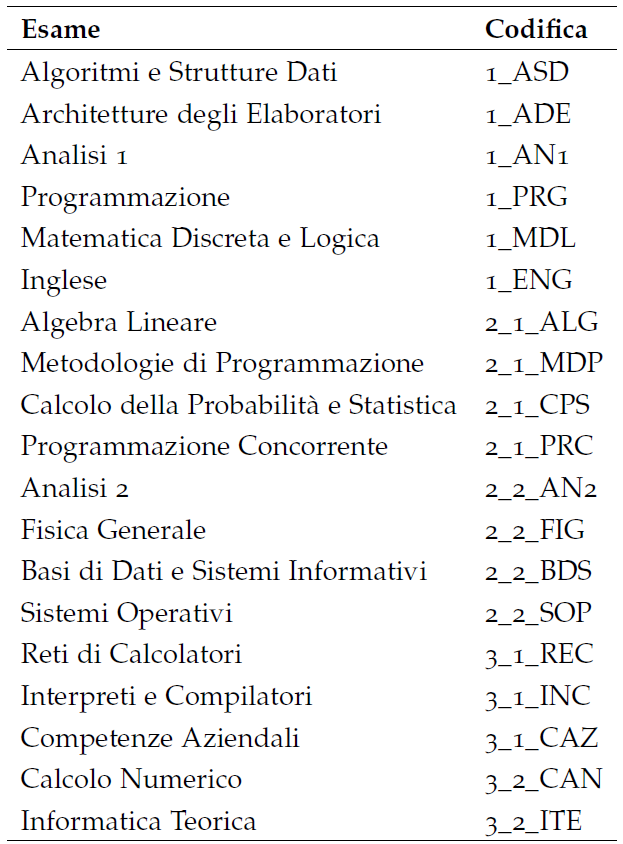
\includegraphics[scale=0.20]{seq1.png}
\end{column}
\begin{column}{0.5\textwidth}
    \hspace*{-0.5cm}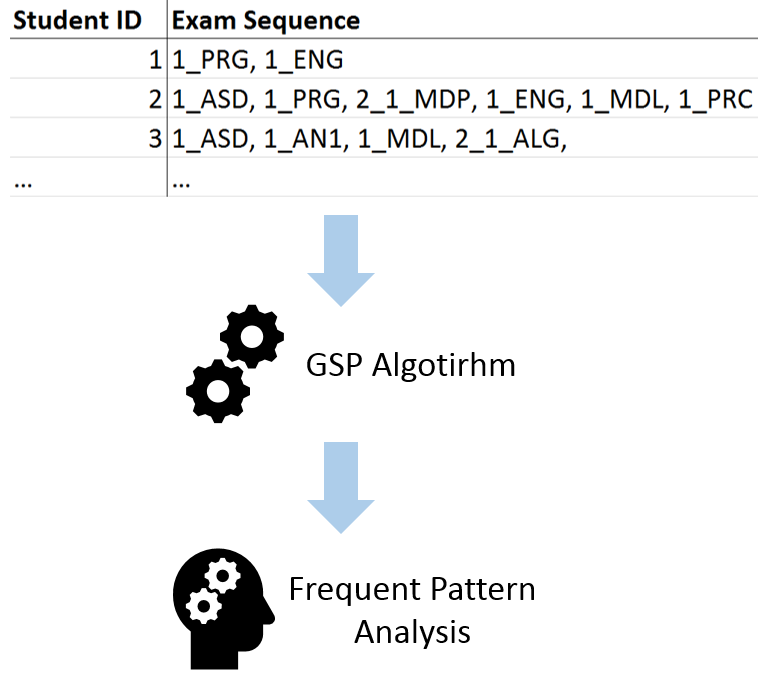
\includegraphics[scale=0.21]{seq3.png}
\end{column}
\end{columns}

\end{frame}

\begin{frame}{Associative Rules Analysis}{Looking for implications among the dataset's attributes}

    \alert{Example} of a \textcolor{cyan}{frequent}, \textcolor{cyan}{unusual} pattern: \\

	\vspace{0.3cm}
	\begin{centering}
		\texttt{3\_2\_CN, 3\_2\_ITE, 2\_2\_FIG}\\
	\end{centering}
	\vspace{0.3cm}

	\ldots which stands for:

	\vspace{0.3cm}
	\begin{centering}
	\texttt{Calcolo Numerico, Informatica Teorica, Fisica Generale}\\
	\end{centering}
	\vspace{0.6cm}

	\texttt{Fisica Generale} is \alert{out of place}, for it is a $2^{nd}$ year exam done after some $3^{rd}$ year exams.\\

\end{frame}

\begin{frame}{Associative Rules Analysis}{Looking for implications among the dataset's attributes}

\vspace{0.1cm}
	Counting how many times an exams is out of place and making proportions with all out-of-place exams, we get...\\ \vspace{0.2cm}

    \begin{centering}
        \hspace*{2cm}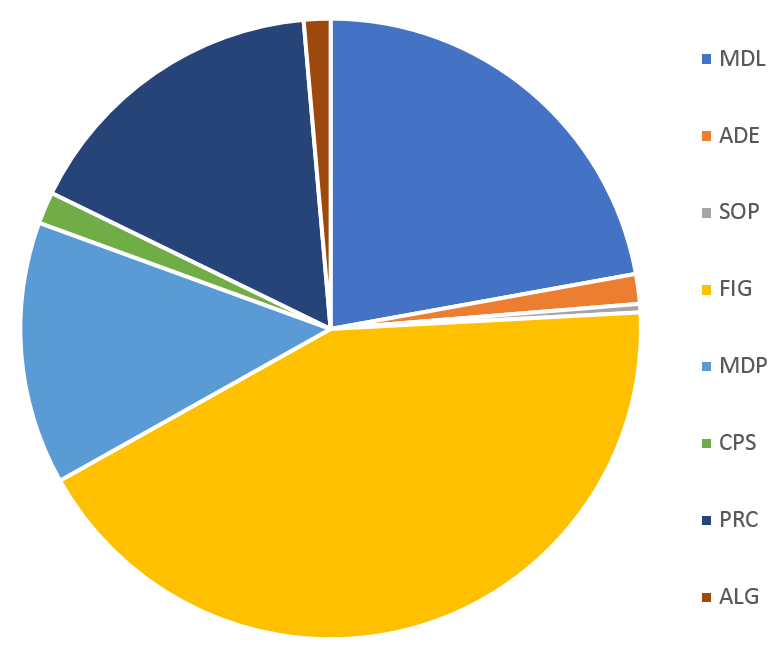
\includegraphics[scale=0.25]{seq2.png}
    \end{centering}

\end{frame}